\documentclass[runningheads]{llncs}
\usepackage[utf8]{inputenc}
\usepackage{setspace}
\usepackage{amssymb}
\usepackage{subfiles}
\usepackage{amsmath}
\usepackage{graphicx}
\usepackage[table,xcdraw]{xcolor}
\usepackage{longtable}
\usepackage[
backend=biber,
style=alphabetic,
giveninits=true
]{biblatex}
\DeclareNameAlias{default}{family-given}
\addbibresource{sources.bib}

\newcommand{\GCP}{{Graph Coloring Problem}\ }

\title{Surveying Cooperative Approaches for the Graph Coloring Problem}
\author{Gabriel Perez
\and
Corey Roberts
\and
Javier Valenzuela
}
\date{\today}

\authorrunning{Perez and Valenzuela and Roberts}

\institute{ Department of Electrical and Computer  Engineering\\
University of Texas at Austin,\\
Austin, TX 78712\\
\email{\{gabriel_ohseas_perez, email2\}@utexas.edu}}

\begin{document}

\def\IEEEQED{\mbox{\rule[0pt]{1.3ex}{1.3ex}}} % for a filled box
\newcommand{\ep}{\hspace*{\fill}~\IEEEQED}
\newenvironment{mproof}[1][Proof]{{\bf #1: }}{\ep\vspace{.1in}}

\maketitle
\doublespacing

\begin{abstract}
  The \GCP is an NP-Complete problem with a rich history of approximation algorithms and heuristics. In this paper, we explore a modification to cooperative local search approaches for the graph coloring problem.
\end{abstract}

\section{Introduction}
The \GCP and its variants are long existing problems with a very low barrier to understanding. Despite that, the class of problems are incredibly difficult problem to solve exactly. Applications of the class of problems include identifying whether a circuit board has a short circuit, solving Sudoku for any size grid, and problems of scheduling exams for university lecturers \cite{10.5555/2851123}.

In this paper, we explore the idea of algorithms with various hyper-parameters cooperating to determine whether we get improved lower bounds for the \GCP approximations.

\section{Definitions}

\subsection{Graph \& Graph Properties}

A graph, $G$, is defined as $G = (V, E)$ a set of $n$ vertices $V$ and $m$ edges $E$. For this class of problems, we have a function $c: V \mapsto \mathbb{N} $. This function is called the \emph{coloring function}. The coloring is \emph{legal} if $\forall (u, v) \in E \implies c(u) \ne c(v)$. If the graph can be colored by using $k$ colors, then the graph is called $k-colorable$. The minimum $k$ that can be used to color the graph $G$ is called the \emph{chromatic number} of the graph $G$ denoted $\chi$. Another important term is neighboring coloring, which involves changing the color of a single vertex.

\subsection{Central Algorithm}

The central algorithm at the heart of these heuristics is to start at $|V|$ colorings, see if a feasible one exists, and then proceed downward. This approach was used for all of the algorithms discussed here. Another key idea used here is the \emph{portfolio} approach, in which we seed the algorithms with various hyper-parameters and consequently reduce

\subsection{Sharing Information}
Throughout this paper, there are references to the term sharing information. It is important to discuss what that precisely means. In this context it is feasible for algorithms to share what the lowest $k$ determined so far is. In addition, it is also feasible for them to share information about what moves they have made. This was the statistic matrix idea suggested by Li. \cite{https://doi.org/10.5445/ir/1000083192} It was implemented for PartialCol algorithm and Tabucol algorithm. It was not performed for the Metropolis algorithm.

\section{Existing Graph Coloring Problem Approaches }

In this section of the paper, we will reference some existing techniques and heuristics for graph coloring as they are vital to understanding the hypothesis.

\subsection{Tabucol \& PartialCol}\label{AA}
Tabucol is an algorithm proposed by Hertz and de Werra \cite{hdw}. The implementation here is the modified version by Galinier and Hao \cite{TabuCol} and discussed in the \emph{Guide to Graph Coloring} textbook \cite{10.5555/2851123}. The algorithm fundamentally revolves around moves, i.e., shifting a coloring to a neighboring coloring by only \emph{moving} the vertex causing the most conflicts to another color class. The algorithm attempts to prevent cyclic issues by making certain moves \emph{taboo} hence the name. The rate at which moves become accessible again is dependent upon algorithm parameters. Another algorithm that was used in this paper is called PartialCol. PartialCol itself is very similar to the tabu approaches, but organizes vertices that cannot be colored without conflict.

\subsection{Metropolis Algorithm}
The metropolis algorithm is a very simple algorithm in which we select vertices, color them, analyze their impact using a cost (or potential) function $H$ (how many neighbors are similarly colored), and approve or reject the color transitioning move with a probability based on the cost of the move. This algorithm also comes with hyper-parameters that are adjustable.

\subsection{Antcol}

Antcol is an algorithm that was proposed by Thompson and Dowsland \cite{ant_kj}. It is an algorithm that utilizes both global and local search operators inspired by how ants determine optimal paths between their colonies and food sources. Ants tend to wander around randomly until a food source is found, where they then leave a pheromone trail for other ants to pick up on. This is key to Antcol: the algorithm attempts to make a handful of individual solutions (i.e. "ants") made in a non-deterministic manner. Then, each individual solution contributes to a global "trail" solution that subsequent "ants" then use as better heuristics. If features identified in each solution lead to better solutions, subsequent ants will continue to use those features using a matrix analogous to an ant's pheromone trail. Over time, inadequate solutions will disappear with an evaporation rate, giving stronger features more prominence.

\section{Cooperative Extensions to the Graph Coloring Problem}

This paper is comprised of several experiments:

\begin{itemize}

  \item Assessing whether one sees improved lower bounds on $\chi$ by running concurrent metropolis algorithms sharing information.
  \item Assessing the performance improvements of of PartialCol and Tabucol sharing lower bounds and partial colorings in identifying lower $\chi$.
  \item Assessing cooperative Tabucol approaches with other algorithms - that is to say extending the results of Li's use of the statistic matrix. \cite{https://doi.org/10.5445/ir/1000083192} The statistic matrix in this scenario is just a means to feature moves that are made less frequently.
  \item Assessing Antcol and tuning hyperparameters in both non-cooperative and cooperative modes. Notably, tuning the evaporation rate and number of ants used to approximate a solution.
\end{itemize}

The source code is available in this project. It was written using a standard Java console application with Gradle for managing dependencies. The most important of those dependencies is JGraphT, an open source library for handling graphs. The graph format that was used is the popular DIMACS format. The graphs used in this project are listed in the appendix in Figure.

\subsection{Cooperative Metropolis Algorithm}

The first experiment was assessing whether we could get better results for Metropolis using multiple threads running different parameters and multiple threads sharing information about what the lowest $k$ currently available is. What was observed is captured in the appendix in Figure \ref{fig:metr1}. What we observed was that we do indeed see a noticeable difference in the minimum coloring achievable. Still, this approach did not yield any significant advances over using different algorithms such as Tabucol and PartialCol, whose results are discussed below.

\subsection{Cooperative Tabucol Algorithm}

The results in Figure \ref{fig:TabuColl} were intended to provide discussion with reference towards \cite{https://doi.org/10.5445/ir/1000083192}. We did find that the portfolio approach decreased the error on our optimal coloring determinations. However, we were fairly surprised that that the statistic matrix approach did not yield significant benefits (in fact, it appeared detrimental). Some possible explanations were listed in the PartialCol section.

\subsection{Cooperative PartialCol Algorithm}

The third experiment performed was analyzing the use of cooperative approaches and the statistic matrix for PartialCol. Again, the surprising result was that the statistic matrix didn't provide any inherent benefit over the standard cooperative approaches or the multithreaded simple portfolio approach. In fact, it performed worse in our experiments. See the average error in Figure \ref{fig:partialcol}.
One possibility is that the implementation by Li had a different synchronization method. Ours was synchronized in access, but not in terms of iterations. Our approach determined that the best approach was simply using a portfolio approach to minimize the odds getting stuck in local minima, as the cooperative approach didn't provide too much overhead.

\subsection{Antcol}

The final experiment performed was assessing Antcol and its hyperparameters: notably, if tuning the number of ants or the evaporation rate of the pheromone matrix would increase or decrease the optimal approximation. The average error for the hyperparameters that were included in \cite{10.5555/2851123} was approximately 0.18. This implementation included an evaporation rate of 0.75. When adjusting this to be higher or lower, we can see based on the graph in \ref{fig:antcol} that lower values of evaporation tended to cater towards lower errors. Specifically, performance for smaller known-colorings proved to reach the optimal coloring. When we experimented using a shared dataset across multiple instances of Antcol, we noticed that the error increased in size. This is likely due to the somewhat random, sequential nature of how Antcol works. Because each individual contribution ends up contributing to the global matrix for each instance, it is possible that a solution set may differ than that of another. While the difference in average error is small, it's worth noting that both increasing the number of ants and lowering evaporation rates improved optimality at an expense in computational effort.

\section{Conclusion}
In this report we examined several different cooperative approaches to various local search algorithms. In addition, we leveraged the novel approach of Li and extended it to the PartialCol algorithm. In the graphs chosen, we did not observe any advantage and in fact saw some distinct disadvantages in terms of average error. For all the algorithms, however, we did see benefit in the portfolio approach. Several other approaches were evaluated (a simple evolutionary algorithm), but we found that they were not performant enough to be viable).


\section{Appendix}

The graphs used are shown below. Optimal is Approximate denotes whether we know a lower bound for said graph.

\begin{longtable}{|l|l|l|l|l|}
  \hline
  \rowcolor[HTML]{F56B00}
  Optimal is Approximate & Optimal Coloring & Graph Name     & Vertices & Edges \\ \hline
  \endhead
%
  F          & 5                & dsjc125.1      & 125      & 736   \\ \hline
  F          & 17               & dsjc125.5      & 125      & 3891  \\ \hline
  F          & 44               & dsjc125.9      & 125      & 6961  \\ \hline
  F          & 8                & dsjc250.1      & 250      & 3218  \\ \hline
  T          & 28               & dsjc250.5      & 250      & 15668 \\ \hline
  F          & 72               & dsjc250.9      & 250      & 27897 \\ \hline
  F          & 26               & flat300\_26\_0 & 300      & 21633 \\ \hline
  F          & 28               & flat300\_28\_0 & 300      & 21695 \\ \hline
  F          & 10               & jean           & 80       & 254   \\ \hline
  F          & 15               & le450\_15b     & 450      & 8169  \\ \hline
  F          & 15               & le450\_15d     & 450      & 16750 \\ \hline
  F          & 5                & le450\_5a      & 450      & 5714  \\ \hline
  F          & 5                & le450\_5b      & 450      & 5734  \\ \hline
  F          & 20               & r1000.1        & 1000     & 14378 \\ \hline
  F          & 5                & r125.1         & 125      & 209   \\ \hline
  F          & 36               & r125.5         & 125      & 3838  \\ \hline
  F          & 8                & r250.1         & 250      & 867   \\ \hline
  F          & 64               & r250.1c        & 250      & 30227 \\ \hline
  T          & 28               & r250.5         & 250      & 14849 \\ \hline
  F          & 14               & school1\_nsh   & 352      & 14612 \\ \hline
  F          & 14               & school1        & 385      & 19095 \\ \hline
\end{longtable}

Note that multithreaded experiments were run with 8 threads. The notation $a[x,y]$ means that parameter $a$ was chosen with arbitrary values between $x$ and $y$. In lieu of $\alpha$ and $\beta$, a and b were used.

\begin{figure}[h]
  \centering
  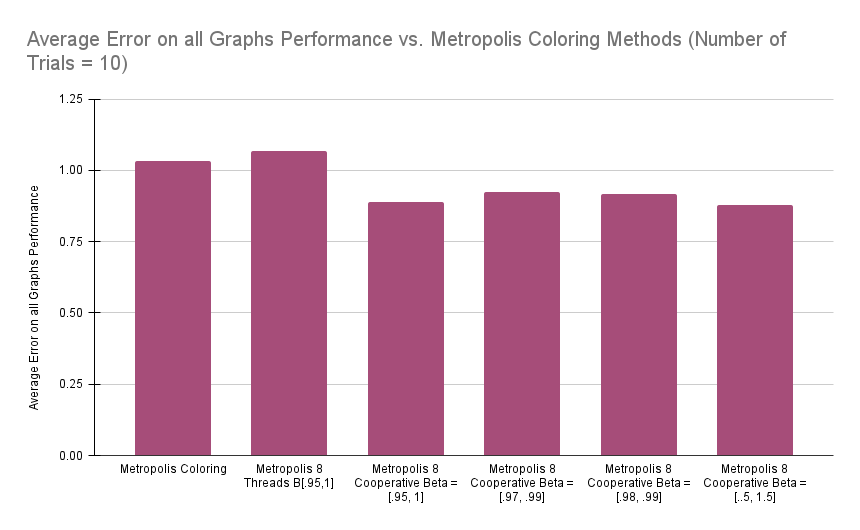
\includegraphics[width=1.125\textwidth]{Metropolis.png}
  \caption{Metropolis Results}
  \label{fig:metr1}
\end{figure}

\begin{figure}[h]
  \centering
  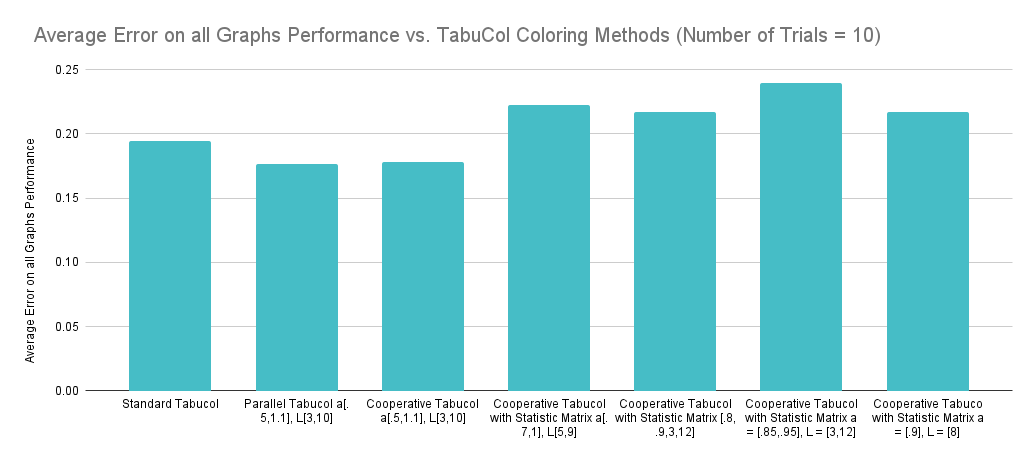
\includegraphics[width=1\textwidth]{Tabucol.png}
  \caption{Tabucol Results}
  \label{fig:TabuColl}
\end{figure}


\begin{figure}[h]
  \centering
  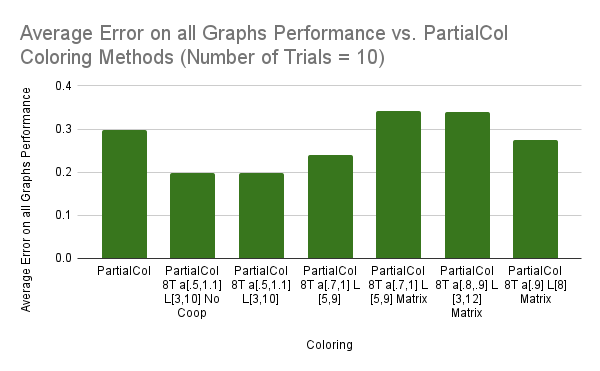
\includegraphics[width=1\textwidth]{PartialCol.png}
  \caption{PartialCol Results}
  \label{fig:partialcol}
\end{figure}

\begin{figure}[h]
  \centering
  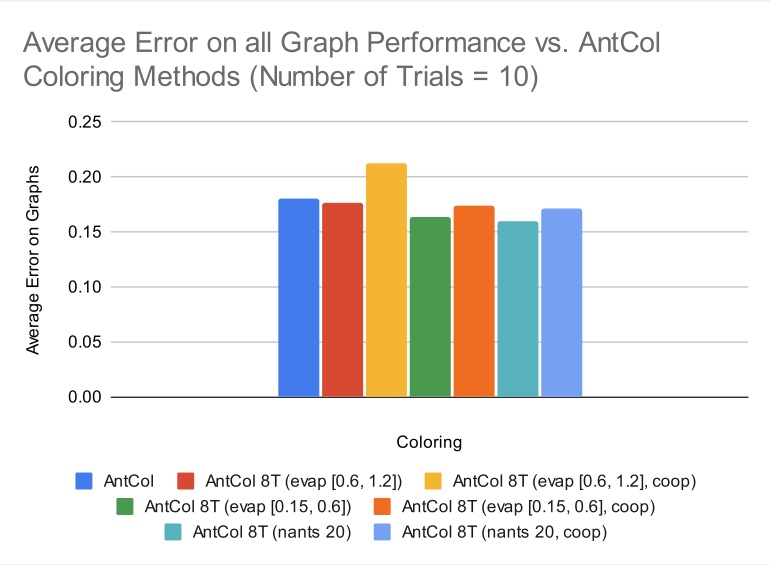
\includegraphics[width=1\textwidth]{AntCol.png}
  \caption{AntCol Results}
  \label{fig:antcol}
\end{figure}


\clearpage

\printbibliography

\end{document}
